\section{Evaluation}
\label{sec:eval}

\subsection{Experimental Settings}
\begin{figure}[h]
  \centering
  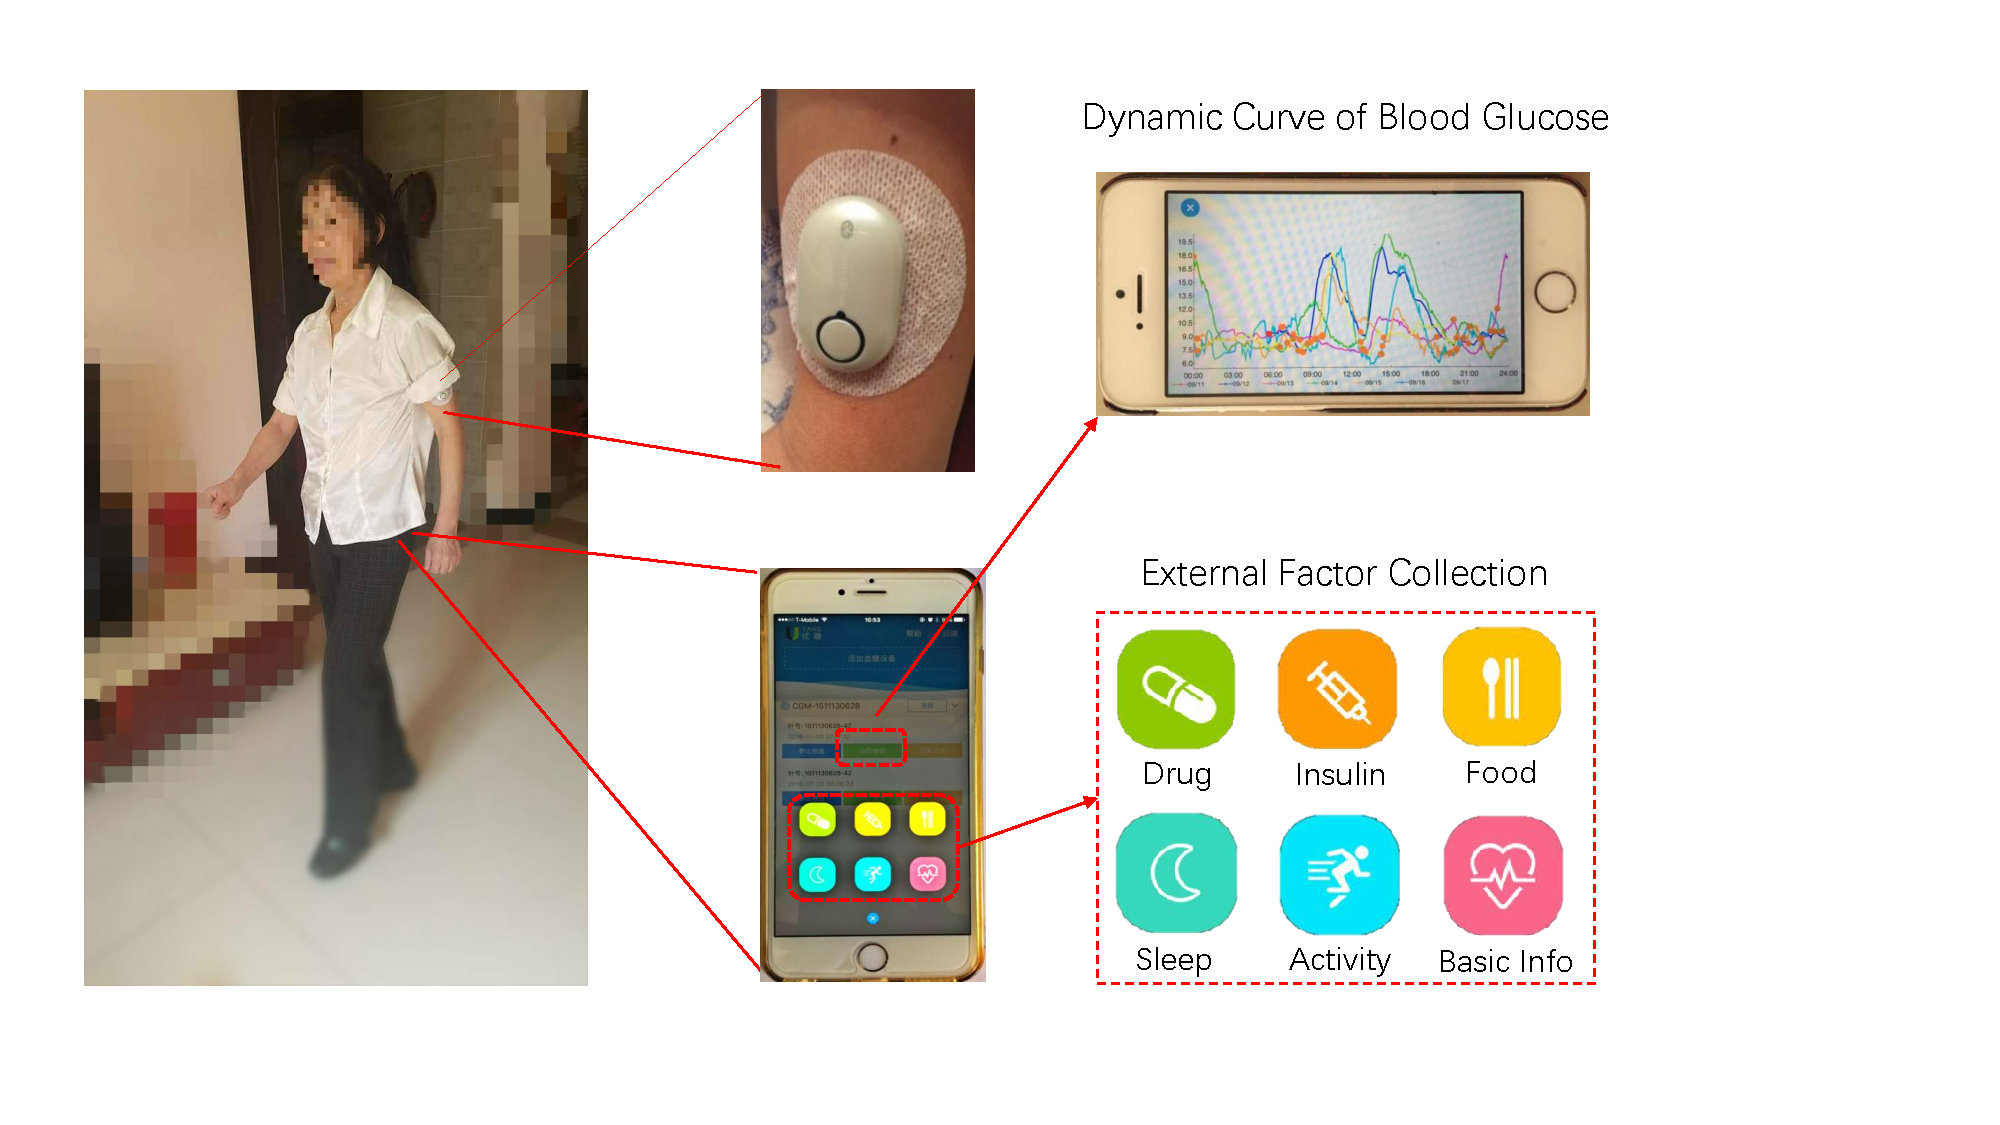
\includegraphics[width=0.7\columnwidth]{./img/UI.pdf}
  \caption{An illustration of the equipments for data collection. Each participant wears a CGM device to record blood glucose concentration and uses a smartphone to collect external factors. }
  \label{fig:experiment_case}
\end{figure}

\textbf{Datasets.}
We validate \sysname on a dataset of $112$ participants ($35$ non-diabetes, $38$ type I diabetic patients and $39$ type II diabetic patients) collected during July 2016 to January 2017.
Each participant is equipped with (1) a WAVEGUIDER \emph{U-Tang} CGM device~\cite{bib:CGM_wave} to record blood glucose concentration every $3$ minutes and (2) a smartphone with \sysname installed to collect external factors either automatically (activities and sleep quality) or manually (food, drug, and insulin intake).
All participants agree to take measurements (\ie wear the CGM device and use \sysname to record external factors) for at least $6$ days, which is a disposable usage duration of enzyme of the CGM.
\figref{fig:experiment_case} illustrates an example of data collection from a user.
In total we obtain 762639 samples of blood glucose concentration and the corresponding external factors covering around 38132 hours.
In brief, we collect the following categories of data:
\begin{itemize}
  \item
  \textbf{Meta information.}
  We record basic personal data including gender, age, weight and health status to cover a wide range of users.
  \tabref{tab:parcitipant} summarizes the basic information of the participants.
  \item
  \textbf{Blood glucose measurements.}
  We collect blood glucose measurements using commercial CGM devices for 6 to 30 days as labeled data.
  \tabref{tab:bgdata} summarizes the blood glucose measurements in our evaluation.
  \item
  \textbf{External factor measurements.}
  During measurements of blood glucose concentration, each participant manually inputs the times of their daily meal, drug and insulin intake.
  \sysname automatically records activity levels and sleep quality as in \secref{subsec:external}.
  \figref{fig:experiment_case} shows the user interfaces to record external factors.
\end{itemize}

\begin{table}
  \centering
  \caption{Summary of participant information.}
  \label{tab:parcitipant}
  \subfloat[]{%
  \begin{tabular}{cc}
  \toprule
  \textbf{Age (year)} & \textbf{\# User} \\
  \midrule
  15-24 & 8 \\
  25-34 & 17 \\
  35-44 & 24 \\
  45-54 & 29 \\
  55-64 & 34 \\
  \bottomrule
  \end{tabular}}%
  \quad% --- set horizontal distance between tables here
  \subfloat[]{%
  \begin{tabular}{ccc}
  \toprule
  \textbf{Weight (kg)} &\textbf{BMI ($kg/m^2$)}\cite{bib:world2013bmi} &\textbf{\# User} \\
  \midrule
  Underweight & (0,  18.5) & 18 \\
  Normal weight & [18.5,  25) & 31 \\
  Overweight &  [25,  30) &41 \\
  Obese &  [30, +$\infty$) & 22 \\
  \bottomrule
  \end{tabular}}%
  \quad%
%  \%subfloat[]{%
%  \begin{tabular}{cc}
%  \toprule
%  \textbf{Status} & \textbf{\# User} \\
%  \midrule
%  Non-diabetes & 35 \\
%  Type I & 38 \\
%  Type II & 39 \\
%  \bottomrule
%  \end{tabular}}
%  \quad%
  \subfloat[]{%
  \begin{tabular}{cc}
  \toprule
  \textbf{Gender} & \textbf{\# User} \\
  \midrule
  Male & 57 \\
  Female & 55\\
  \bottomrule
  \end{tabular}}
\end{table}

\begin{table}
  \centering
  \caption{Summary of blood glucose measurements.}
  \label{tab:bgdata}
  \subfloat[]{%
  \begin{tabular}{cc}
  \toprule
  \textbf{Duration (days)} & \textbf{\# User} \\
  \midrule
  6-10 & 48 \\
  11-15 & 24 \\
  16-20 & 20 \\
  21-25 & 13 \\
  26-30 & 7 \\
  \bottomrule
  \end{tabular}}%
  \qquad% --- set horizontal distance between tables here
  \subfloat[]{%
  \begin{tabular}{cc}
  \toprule
  \textbf{Blood Glucose} & \textbf{\# Sample} \\
  \midrule
  Level 1 & 75369 \\
  Level 2 & 293530 \\
  Level 3 & 235686 \\
  Level 4 & 158054 \\
  Total & 762639 \\
  \bottomrule
  \end{tabular}}%
\end{table}

%\begin{table}[]
%  \centering
%  \caption{Summary of experimental settings.}
%  \label{tab:dataset}
%  \begin{tabular}{clccclcccccl}
%  \hline\hline
%  \multicolumn{12}{c}{\textbf{Blood Glucose}}                                                                                                                                                                                               \\ \hline
%  \multicolumn{2}{l}{\textbf{\cellcolor[gray]{0.8}Blood Level}} & \multicolumn{2}{r}{\textbf{\cellcolor[gray]{0.8}Level 1}} & \multicolumn{2}{c}{\textbf{\cellcolor[gray]{0.8}Level 2}} & \multicolumn{2}{c}{\textbf{\cellcolor[gray]{0.8}Level 3}} & \multicolumn{2}{c}{\textbf{\cellcolor[gray]{0.8}Level 4}} & \multicolumn{2}{c}{\textbf{\cellcolor[gray]{0.8}Total}} \\
%  \multicolumn{2}{l}{Number of Sample}     & \multicolumn{2}{c}{75369}            & \multicolumn{2}{c}{293530}           & \multicolumn{2}{c}{235686}           & \multicolumn{2}{c}{158054}           & \multicolumn{2}{c}{762639}         \\ \hline\hline
%  \multicolumn{12}{c}{\textbf{Experimental Duration}}                                                                                                                                                                                          \\ \hline
%  \multicolumn{2}{l}{\textbf{\cellcolor[gray]{0.8}Days}}        & \multicolumn{2}{c}{\textbf{\cellcolor[gray]{0.8}6-10}}    & \multicolumn{2}{c}{\textbf{\cellcolor[gray]{0.8}11-15}}   & \multicolumn{2}{c}{\textbf{\cellcolor[gray]{0.8}16-20}}   & \multicolumn{2}{c}{\textbf{\cellcolor[gray]{0.8}21-25}}   & \multicolumn{2}{c}{\textbf{\cellcolor[gray]{0.8}26-30}} \\
%  \multicolumn{2}{l}{Number of Users}      & \multicolumn{2}{c}{48}               & \multicolumn{2}{c}{24}               & \multicolumn{2}{c}{20}               & \multicolumn{2}{c}{13}               & \multicolumn{2}{c}{7}              \\
%  \hline\hline
%  \multicolumn{12}{c}{\textbf{Summary of participant data}}                                                                                                                                                                                      \\ \hline
%  \multicolumn{2}{l}{\textbf{\cellcolor[gray]{0.8}Age}}         & \multicolumn{2}{c}{\textbf{\cellcolor[gray]{0.8}15-24}}   & \multicolumn{2}{c}{\textbf{\cellcolor[gray]{0.8}25-34}}   & \multicolumn{2}{c}{\textbf{\cellcolor[gray]{0.8}35-44}}   & \multicolumn{2}{c}{\textbf{\cellcolor[gray]{0.8}45-54}}   & \multicolumn{2}{c}{\textbf{\cellcolor[gray]{0.8}55-70}} \\
%  \multicolumn{2}{l}{Number of Users}      & \multicolumn{2}{c}{8}                & \multicolumn{2}{c}{17}               & \multicolumn{2}{c}{24}               & \multicolumn{2}{c}{29}               & \multicolumn{2}{c}{34}             \\
%  \multicolumn{2}{l}{\textbf{\cellcolor[gray]{0.8}Weight}}      & \multicolumn{2}{c}{\textbf{\cellcolor[gray]{0.8}30-44}}   & \multicolumn{2}{c}{\textbf{\cellcolor[gray]{0.8}45-54}}   & \multicolumn{2}{c}{\textbf{\cellcolor[gray]{0.8}55-64}}   & \multicolumn{2}{c}{\textbf{\cellcolor[gray]{0.8}65-74}}   & \multicolumn{2}{c}{\textbf{\cellcolor[gray]{0.8}75-90}} \\
%  \multicolumn{2}{l}{Number of Users}      & \multicolumn{2}{c}{18}               & \multicolumn{2}{c}{21}               & \multicolumn{2}{c}{32}               & \multicolumn{2}{c}{22}               & \multicolumn{2}{c}{19}             \\
%  \multicolumn{4}{l}{\textbf{\cellcolor[gray]{0.8}Gender}}      & \multicolumn{3}{c}{\textbf{\cellcolor[gray]{0.8}Male}}                                                               & \multicolumn{5}{c}{\textbf{\cellcolor[gray]{0.8}Female}}                                                          \\
%  \multicolumn{4}{l}{Number of Users}      & \multicolumn{3}{c}{57}                                                                          & \multicolumn{5}{c}{55}                                                                       \\ \hline\hline
%  \multicolumn{12}{c}{\textbf{User Health Status}}                                                                                                                                                                                          \\ \hline
%  \multicolumn{3}{l}{\textbf{\cellcolor[gray]{0.8}Health Status}}                   & \multicolumn{3}{c}{\textbf{\cellcolor[gray]{0.8}Health}}                     & \multicolumn{3}{c}{\textbf{\cellcolor[gray]{0.8}Type I}}                      & \multicolumn{3}{c}{\textbf{\cellcolor[gray]{0.8}Type II}}                  \\
%  \multicolumn{3}{l}{Number of Users}                          & \multicolumn{3}{c}{35}                                  & \multicolumn{3}{c}{38}                                   & \multicolumn{3}{c}{39}                                \\ \hline
%  \end{tabular}
%\end{table}

\textbf{Ground Truth.}
We use the blood glucose concentrations collected by the CGM device as ground truth \footnote{While clinical studies report that the precision and accuracy of commercial CGM devices still need improving~\cite{bib:MEP08:Do, bib:JDST10:Vaddiraju}, they are sufficient as ground truth for the four normal and abnormal blood glucose levels.}.

\textbf{Metrics.}
We mainly adopt precision, recall and accuracy~\cite{prf1} to quantify the performance of \sysname.
%
%
%\begin{table}[]
%\centering
%\caption{The details of dataset}
%\label{The details of dataset}
%\begin{tabular}{|l|c|c|c|c|l|}
%\hline
%\textbf{Blood Level}                  & \textbf{Level 1} & \textbf{Level 2} & \textbf{level 3} & \textbf{Level 4} & \textbf{Total}         \\ \hline
%\multicolumn{1}{|c|}{\textbf{Number}} & 75369            & 293530           & 235686           & 158054           & \multicolumn{1}{c|}{762639} \\ \hline
%\end{tabular}
%\end{table}


\subsection{Inference Accuracy}
\subsubsection{Overall Inference Accuracy}
Since all participants collected both measurements of CGM and external factors for at least 6 days, \ie a normal usage duration of enzyme in the CGM, we use measurements during the former 5 days for training and the rest for testing.
\tabref{tab:confusion_matrix} shows the overall performance of \sysname.
All results are averaged over the testing data.
As shown, the recalls and the precisions for all the 4 blood glucose levels are above 79\% and 73\%, respectively.
In particular, the recalls for Level 1 (low blood glucose) and Level 4 (high blood glucose) are 83.13\% and 85.23\%, even though the training data for Level 1 and Level 4 only take up 9.88\% and 20.72\% of the entire training set.
This result shows that \sysname can accurately infer low/high blood levels even with an imbalanced training dataset.
Overall, \sysname yields an accuracy of 82.14\%, showing a promising performance to track blood glucose levels.

\begin{table}[h]
  \centering
  \caption{Confusion matrix of \sysname.}
  \label{tab:confusion_matrix}
  \begin{tabular}{|c|c|c|c|c|l|l|}
  \hline
  \multirow{2}{*}{\textbf{\begin{tabular}[c]{@{}c@{}}Ground\\ Truth\end{tabular}}} & \multicolumn{4}{c|}{\textbf{Inference}}                                                                                 & \multicolumn{2}{l|}{\multirow{2}{*}{}}                                                            \\ \cline{2-5}
                                                                                 & Level 1                      & Level 2                      & Level 3                      & Level 4                      & \multicolumn{2}{l|}{}                                                                             \\ \hline
Level 1                                                                          & \cellcolor[gray]{0.8}62657                        & 5521                         & 3672                         & 3519                         & 83.13\%                             & \multirow{4}{*}{\rotatebox{90}{\textbf{Recall}} }                           \\ \cline{1-6}
Level 2                                                                          & 16346                        &  \cellcolor[gray]{0.8}240584                       & 27563                        & 9037                         & 81.96\%                             &                                                             \\ \cline{1-6}
Level 3                                                                          & 2660                         & 30905                        & \cellcolor[gray]{0.8}188472                       & 13649                        & 79.97\%                             &                                                             \\ \cline{1-6}
Level 4                                                                          & 3443                         & 5620                         & 14278                        & \cellcolor[gray]{0.8}134713                       & 85.23\%                             &                                                             \\ \hline
\multicolumn{1}{|l|}{\multirow{2}{*}{}}                                          & \multicolumn{1}{l|}{73.62\%} & \multicolumn{1}{l|}{85.12\%} & \multicolumn{1}{l|}{80.55\%} & \multicolumn{1}{l|}{83.72\%} & \multicolumn{2}{l|}{\multirow{2}{*}{\begin{tabular}[c]{@{}l@{}}Accuracy:\\ 82.14\%\end{tabular}}} \\ \cline{2-5}
\multicolumn{1}{|l|}{}                                                           & \multicolumn{4}{c|}{\textbf{Precision}}                                                                                 & \multicolumn{2}{l|}{}                                                                             \\ \hline
\end{tabular}
\end{table}


\subsubsection{Inference Result Analysis}
\label{subsec:predict_result_analysis}
To understand the inference accuracy and the risks of different types of errors in the context of blood glucose management, we classify the inference results based on the Clarke Error Grid Analysis (CEGA) \cite{bib:DTT05:Clarke}.
The analysis classifies the inference results into correct event (Type A) and different types of errors (Type B to Type E) with increasing levels of severity.
For instance, Type B errors are those that will not lead to inappropriate treatments, while Type E errors can lead to wrong treatment.
\tabref{predict_results} summarizes the percentages of each type of results.
As shown, \sysname will not cause inappropriate treatment (Type A and B) in almost 90\% of the cases.
It may lead to unnecessary worries or treatment (Type C) in 5.47\% of the cases.
In fewer than 5\% of the cases, \sysname will miss an abnormal blood glucose event (Type D) or confuse treatment (Type E).
Therefore, \sysname is suitable as an temporal alternative for CGM devices.
However, we do not recommend \sysname for extended duration of usage for patients serious diabetics, who need regular blood glucose management.

\small
\begin{table}[h]
\centering
\caption{Inference Result Analysis}
\label{predict_results}
\begin{tabular}{|c|l|c|}
\hline
\textbf{Type of Result} & \multicolumn{1}{c|}{\textbf{Explanation of Result}}                                                                                                                                                                                                & \textbf{Percentage} \\ \hline
Type A                  & \begin{tabular}[c]{@{}l@{}}The inference value is consistent with the true value.\\ (\ie the inference blood glucose level is correct.)\end{tabular}                                                                                             & 82.14\%             \\ \hline
Type B                  & \begin{tabular}[c]{@{}l@{}}The inference result would not lead to inappropriate treatment. \\ (\ie Level 2 is predicted as Level 3, or vice-versa.)\end{tabular}                                                                                 & 7.67\%              \\ \hline
Type C                  & \begin{tabular}[c]{@{}l@{}}The inference result will lead to unnecessary treatment. \\ (\emph{i.e.}, Level 2 is predicted as Level 1/4,or Level 3 is predicted as Level 1/4.)\end{tabular}                                                                       & 5.47\%              \\ \hline
Type D                  & \begin{tabular}[c]{@{}l@{}}Fail to detect hypoglycemia or hyperglycemia.\\ (\ie Level 1/4 are predicted as Level 2/3.)\end{tabular} & 3.81\%              \\ \hline
Type E                  & \begin{tabular}[c]{@{}l@{}}The predicted results that would confuse treatment by mistaking hypoglycemia\\ for hyperglycemia or vice-versa.\\ (\ie Level 1 is predicted as Level 4, and vice-versa.)\end{tabular}                                           & 0.91\%              \\ \hline
\end{tabular}
\end{table}


\subsubsection{Temporal View of Inference Results}
\figref{fig:pre_gt} plots the example inference results of \sysname of three participants (one non-diabetic, one Type I diabetic patient, and one Type II diabetic patient) throughout a day.
The errors are depicted at the bottom of each figure.
As shown, the true blood glucose levels vary during the day after important daily activities such as food intake (5:00, 11:30 and 19:00 for the non-diabetic user; 6:00 and 16:50 for the type I diabetic user; 6:00, 12:50 and 17:45 for the type II user), insulin injection (7:30 for the type I diabetic user), drug intake (15:10 for the type II user) and exercises (15:30 for the type II user), indicating the importance of external factors.
The blood glucose levels inferred by \sysname also match the true blood glucose levels most of the time, which validates the effectiveness of \sysname during various daily activities.

Most errors mistake adjacent blood glucose levels, and usually occur during the transition of two blood glucose levels (\eg from 6:00 to 6:30 for the type II user), or in case of sudden blood glucose concentration change (\eg at 2:30 for the non-diabetic user and at 0:30 for the type I user).
Errors during blood glucose transitions are mainly caused by the delays to measure the external factors.
Errors in case of sudden blood glucose changes occur because the sudden changes in blood glucose concentration may not immediately result in sudden changes in the external factors.
Nevertheless, both errors tend to occur for a short duration of time, which will not lead to risky emergencies.


%For the former one, it is mainly due to the external factors tracked by \modelname have just changed for a short time, resulting in a little temporal delay to follow the true values. This type of error, however, can be revised quickly.
%For the latter one, the period of sudden blood glucose fluctuation lasts too short for \sysname to detect the dynamics of external factors. Nevertheless, the duration of this kind of error is too short, which hardly harm the users.

%\textcolor[rgb]{1.00,0.00,0.00}{Moreover, we can also learn most of errors belongs to the Type B/C  rather than Type D/E (serious error) in the \tabref{predict_results}, which are also accordant with the conclusion in \secref{subsec:predict_result_analysis}.}

\begin{figure}[h]
  \centering
  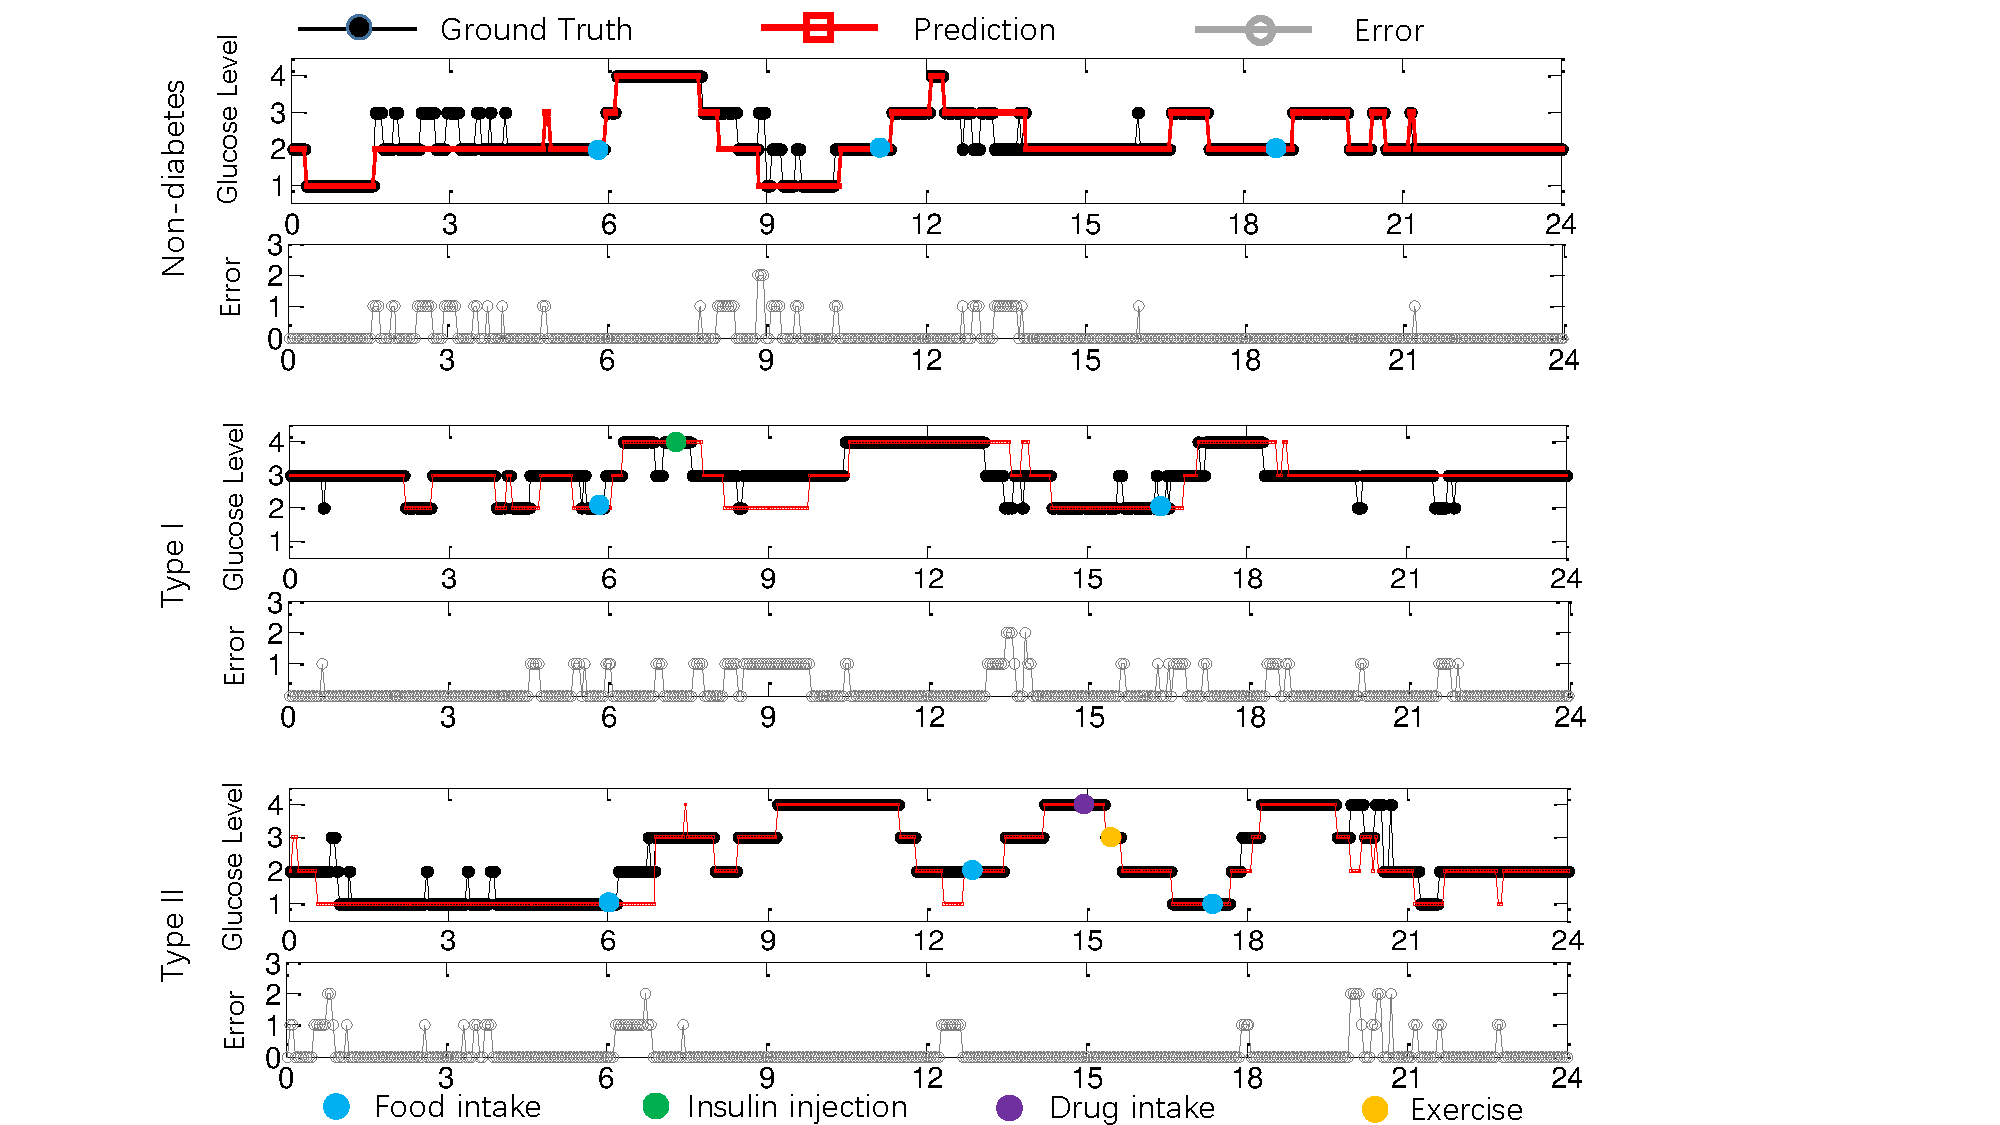
\includegraphics[width=0.8\columnwidth]{./img/pred_vs_gt2.pdf}
  \caption{Traces of blood glucose level inference results throughout a day.}
  \label{fig:pre_gt}
\end{figure}

\subsection{Model Comparison}

\subsubsection{Effectiveness of Multi-division Framework}
To demonstrate the effectiveness of the multi-division framework in making full use of the training dataset, we evaluation \modelname from two perspectives.

\fakeparagraph{Layer contribution analysis}
To evaluate the effect of different layers, we conduct blood glucose level inference with three combinations of layers.
\begin{itemize}
  \item
  \emph{Deep dynamic layer.}
  Training without considering differences in groups and only output a general model.
  \item
  \emph{Grouped input layer + deep dynamic layer.}
  Learn group-specific feature representations but ignore per-person characteristics in the output.
  \item
  \emph{Grouped input layer + deep dynamic layer + personalized output layer (\modelname).}
  Efficiently learn features from different groups and output personalized inference results.
\end{itemize}
\figref{fig:cmp_model} plots the comparison results of the three combinations.
As shown, both the precisions and recalls increase with more layers, with an improvement of 21.13\% in average precision and 18.57\% in average recall, respectively.
Moreover, the standard deviations drop remarkably from 17.25\% to 10.25\%  of average precision, and from 20.75\% to 10.75\% of average recall.
The results demonstrate the effectiveness of \modelname, which learns representative features from the same groups and considers individual differences in blood glucose level inference.

\begin{figure}[h]
  \centering
  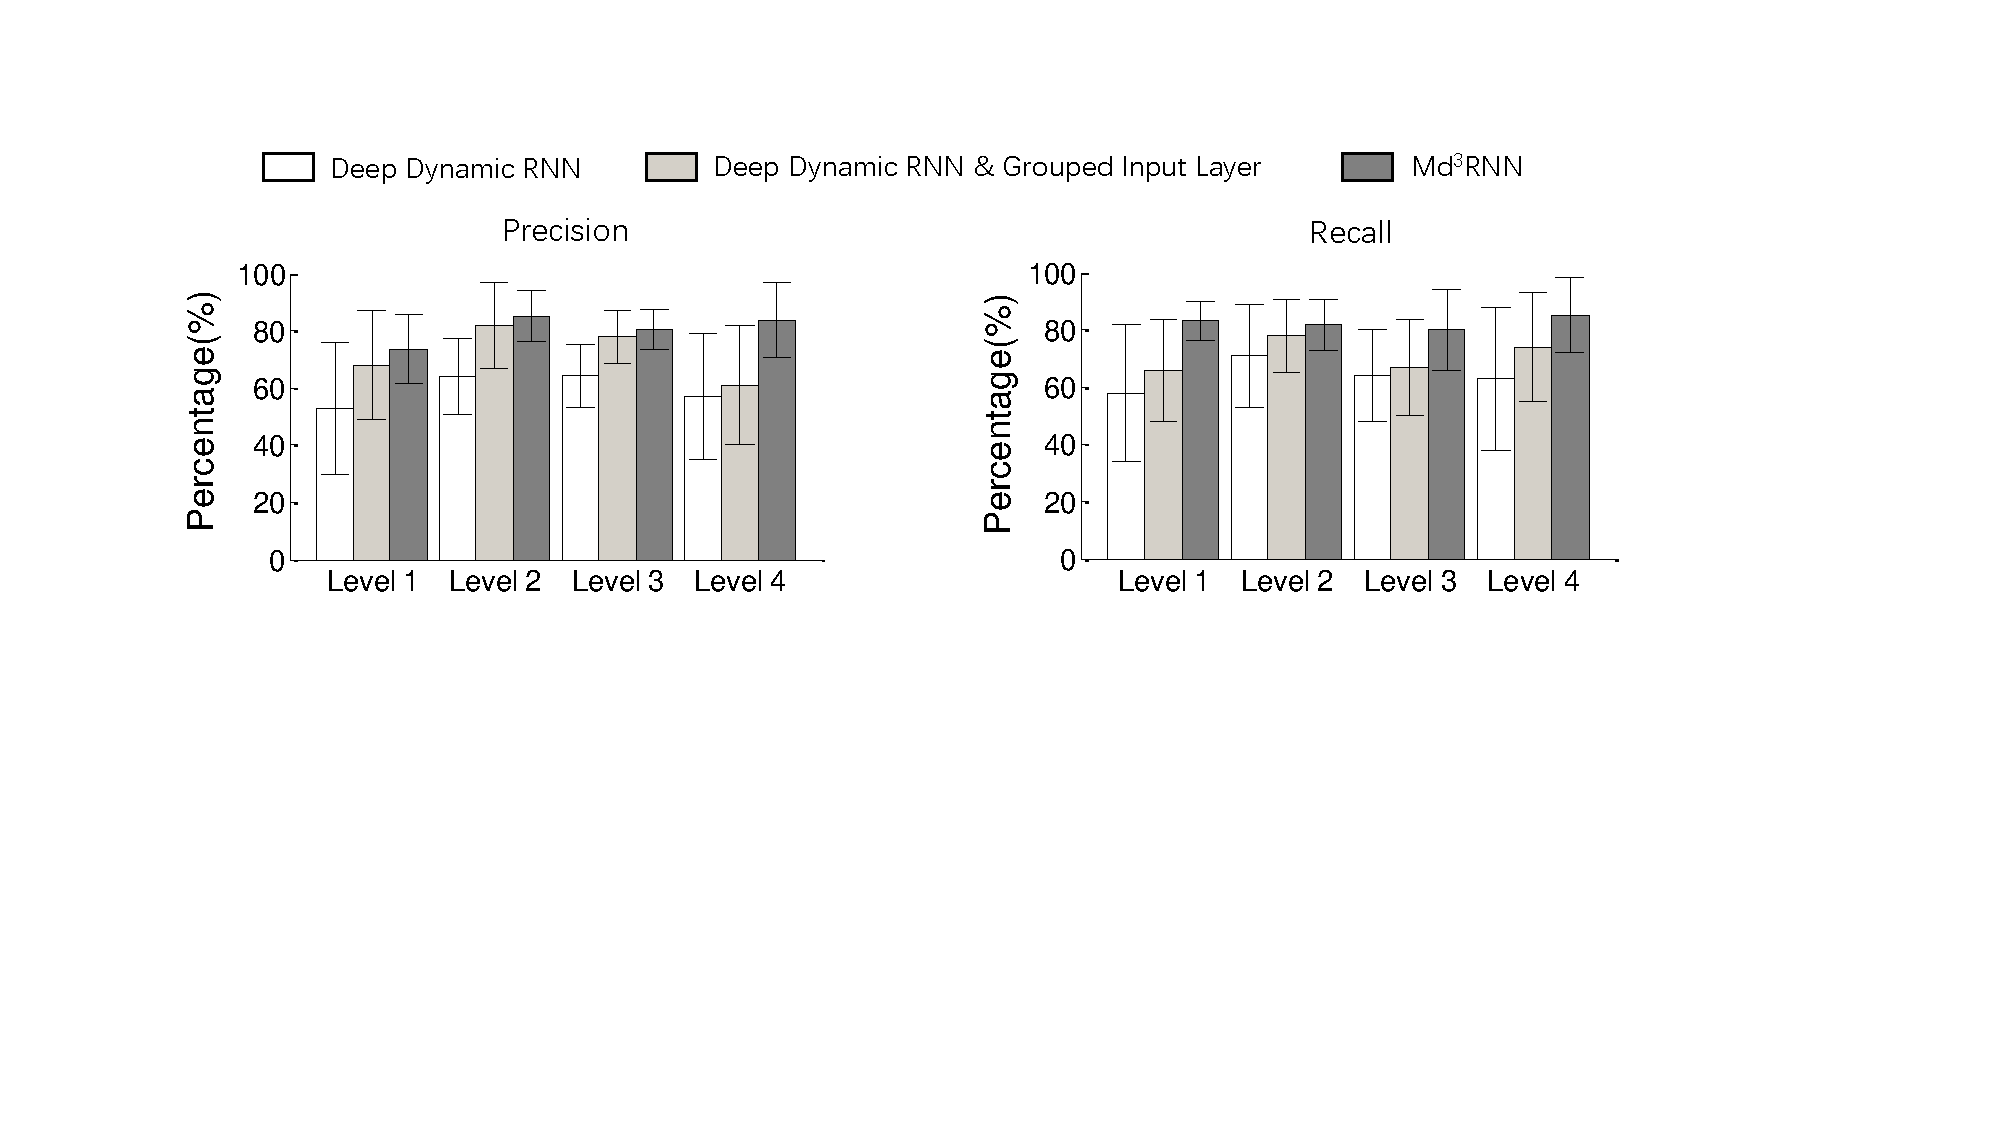
\includegraphics[width=0.9\columnwidth]{./img/CMP_Models1.pdf}
  \caption{Performance of layer combinations.}
  \label{fig:cmp_model}
\end{figure}

\fakeparagraph{Comparison of data sharing schemes}
To demonstrate the benefits of sharing data and knowledge among groups and users, we compare \modelname with other learning frameworks with different data sharing schemes.
\begin{itemize}
  \item \emph{General Learning.}
  All the training data are directly fed into the model (\ie deep RNN) for training indifferently.
  General learning results in a \emph{generic} model that assumes universal correlations between all inputs and the blood glucose levels.
  \item \emph{Group Learning.}
  The data of users belonging to a same group are fed into a model (\ie deep RNN) for training.
  Three separate models are obtained for three groups (\ie non-diabetic, type I and type II diabetic).
  The group learning results in a \emph{group} model that shares the general characteristics of users within the same group but without data sharing among users in different groups.
  \item \emph{Single Learning.}
  We train a different model (\ie deep RNN) for each individual participant by feeding his/her own measurements into the model.
  Single learning results in a \emph{personalized} model without sharing data and learning knowledge from measurements of other participants.
\end{itemize}

\figref{fig:cmp_multi_division} shows the overall precisions and recalls of our \modelname as well as \emph{General learning}, \emph{Group learning} and \emph{Single learning}.
As shown, our multi-divisional learning framework (\modelname) performs best among the four learning approaches with an average precision of 80.75\% and an average recall of 82.57\%.
It also yields the lowest standard deviations (17.18\% of average precision and 17\% of average recall).
The results show that \modelname is both effective and stable in blood glucose level inference.

General learning treats each sample of training data equally, and ignores the individual differences, so it performs poorly in most cases.
Conversely, single learning approach encodes the individual characteristics but suffers from lacking of user-specific training dataset. Even though group learning learns the similarities of users within the same group, it ignores inter-person physiological differences.
\modelname combines the advantages of these three learning approaches, which makes better use of the limited training data by sharing measurements among users and preserves user-specific characteristics via the personal learning layer.

%General learning performs slightly better than single learning for Level 2 and 3 (normal blood glucose levels), partly because the correlations between the inputs and normal blood glucose levels are relatively consistent for most people, while single learning suffers from lack of training data as it only uses user-specific data.
%Conversely, single learning achieves higher precision and recall than general learning for Level 1 and 4 (abnormal blood glucose levels), partly because there are notable inter-person differences in the correlations between the inputs and abnormal blood glucose levels.
%That is, the reasons for abnormal blood glucose levels can vary from person to person.


\begin{figure}[h]
  \centering
  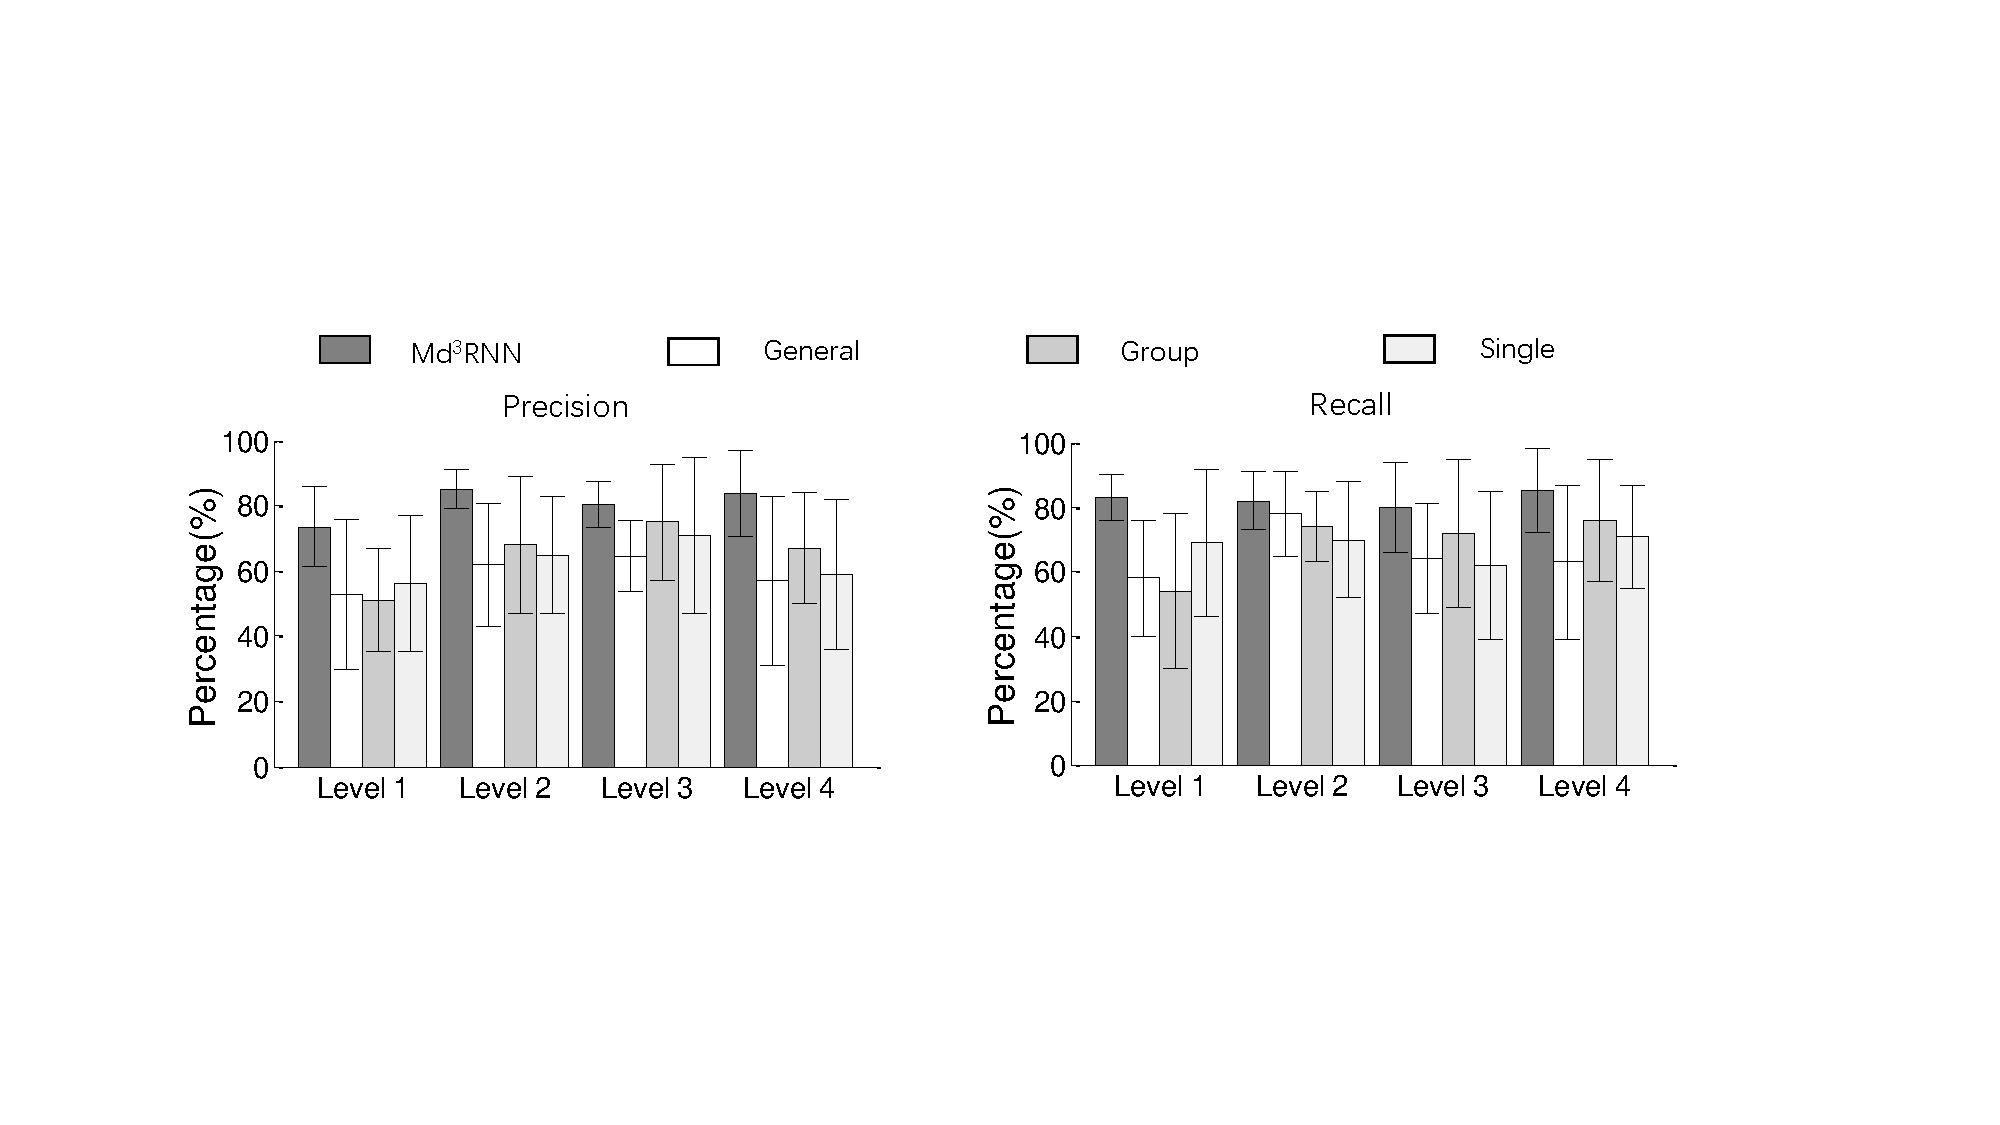
\includegraphics[width=0.9\columnwidth]{./img/performance_of_multi_division.pdf}
  \caption{Performance comparison of different data sharing schemes.}
  \label{fig:cmp_multi_division}
\end{figure}


\subsubsection{Effectiveness of Deep, Multi-division Learning}
To demonstrate the effectiveness of adopting deep learning algorithms over conventional shallow learning algorithms, we compare our \modelname with the following algorithms.
\begin{itemize}
  \item
  \textbf{Gradient Boosting (GB).}
  GB \cite{bib:friedman2002stochastic} generates a prediction model by combining many weak classifiers into a stronger classification committee.
  We use AdaBoost procedure implemented in the fastAdaboost package to combine basic tree classifiers for ensemble learning.
  %We vary the maximum tree depth from 10 to 50 by factors of ten.
  %The number of boosting iterations is varied from 100 to 500 by a step size of 50.
  \item
  \textbf{Support Vector Machine (SVM).}
  SVM \cite{bib:wang2005support} bases on the idea of ��optimal separating hyperplane�� that maximizes the separation margin of two data groups (classes).
  Due to this construction, it usually generalizes well, and its dual form is a quadratic programing that can be easily incorporated with kernels.
  We train the Gaussian kernel SVM classifier with the kernlab package, which implements the sequential minimal optimization algorithm.
  %We vary the kernel width from $2^{-5}$ to $2^4$ with a factor of 2.
  %We pick the penalty parameter from the set $\{10^i | i = -3, 0.5, 2\}$.
  To eliminate scale/location discrepancies among input variables, all features are normalized before being used in the training phase.
  \item
  \textbf{Hidden Markov model (HMM).} \cite{bib:rabiner1986introduction}
  Being a classical example of dynamic Bayesian networks, HMM assumes that the observed process is driven by a hidden (unobserved) Markovian process. Simple as it is, HMM is widely used in signal processing and time series analysis due to its flexibility and tractability. In addition, it has close tights with optimal filtering and state estimation. In our implementation, HMM is learned with the classic Viterbi algorithm. 
  \item
  \textbf{Artificial neural network (ANN).}\cite{bib:wang2003artificial}
  We also included the classical ANN as a baseline, simply to justify the benefit of ``structure engineering'' from \modelname. The ANN under comparison contains a single input layer, three hidden layers, and an output layer. The training of ANN is done by using the stochastic gradient descend algorithm implemented in Tensorflow.  
  \item
  \textbf{Random Forest (RF).}
  As another ensemble method, RF~\cite{bib:liaw2002classification} combines many simple decision trees together and output the mode of classes for prediction.
  To avoid correlation among base trees, random set of features are selected in the splitting process when constructing each decision tree.
  For implementation, we adopt the conditional inference tree algorithm in the Party package.
  %The total number of trees is tuned from 100 to 1000, and the maximum tree depth from 10 to 50.
  %The splitting threshold is also varied from 0.1 to 0.9 with 0.1 intervals for cross validation.
  \item
  \textbf{Gaussian Processes (GP).}
  Instead of directly parameterizing a latent function for classification, GP~\cite{bib:rasmussen2006gaussian} models it with a generic Gaussian process.
  The posterior of the process is updated with training data set, and is ``squashed'' through a logistic function for classification.
  We implement GP with the kernlab package, which includes several approximation algorithms for acceleration.
  %We use the radial basis kernel and vary the kernel width from 2$^{-5}$ to 2$^4$ with an incremental factor of 2$^{0.5}$.
\end{itemize}

\figref{fig:cmp_models} illustrates the results.
Apparently, \modelname achieves best performance on both precisions and recalls.
More specifically, it outperforms the runner-up by at least 20\% in terms of precision, and yields much better recalls for the categories of interest, i.e., level 1 and level 4. Among those baselines, it appears that no method could dominate the others, except that HMM performs slightly better in terms of recall score. This is mainly because HMM is the only method among baselines that incorporates temporal dependence. However compared to \modelname which is able to describe multi-scale dynamics, overall HMM is still much worse.  The overwhelming performance of \modelname is somewhat expected, as those classical baselines either ignore the multi-scale dynamics of the observed data, or does not allow information sharing among available data from grouped users. The above observation further justifies the effort of adopting valuable knowledge about the application, for the design of new machine learning paradigms. 
\begin{figure}[h]
  \centering
  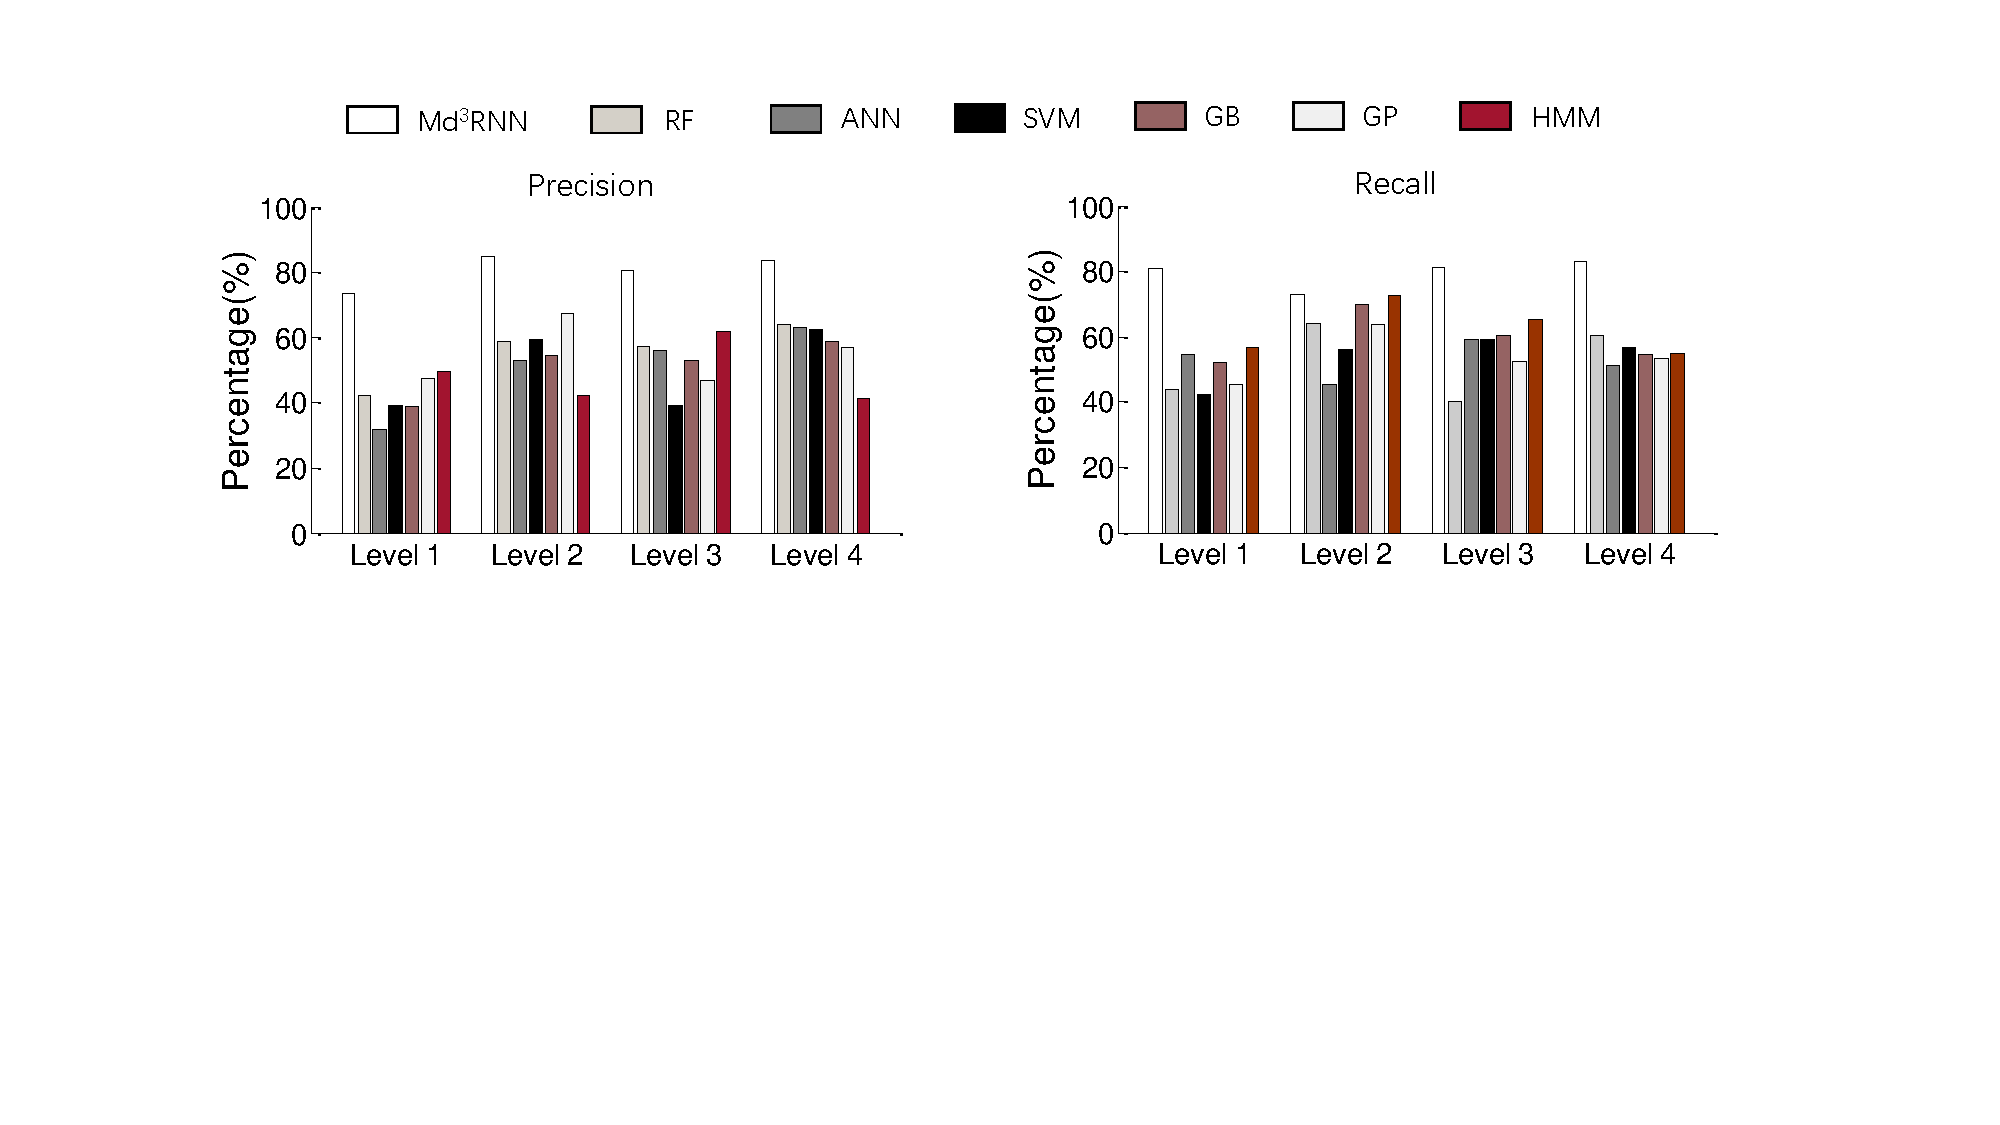
\includegraphics[width=0.9\columnwidth]{./img/Model_CMP.pdf}
  \caption{Performance comparison with shallow learning algorithms.}
  \label{fig:cmp_models}
\end{figure}




%It was then used to quantify the clinical accuracy of blood glucose estimates generated by meters as compared to a reference value.

\subsection{Micro-benchmarks}
\subsubsection{Effectiveness of Features}
\tabref{tab:features} shows the average precisions and recalls for all the 4 blood glucose levels with different combinations of features.
By combining physiological features ($X_{P}$) with temporal features ($X_{T}$), the average precision and recall of the 4 blood glucose levels improve by 31.38\% and 41.48\%, respectively.
Specifically, the physiological features ($X_{P}$) and the historical blood glucose trend ($X_{T_1}$) bring in the most notable improvement in detecting abnormal blood glucose events (Level 1 and Level 4).
This is because the physiological model can well describe the impact of external factors (\eg food and exercise), and the historical trend enables to track the individual temporal dynamics of average blood glucose concentrations in recent time. 

\begin{table}[h]
  \small
  \centering
  \caption{Effectiveness of features.\TODO{no $X_{T_2}$ now.}}
  \label{tab:features}
  \begin{tabular}{|c|c|c|c|c|c|c|c|c|}
  \hline
                                   & \multicolumn{2}{c|}{\textbf{Level 1}}                     & \multicolumn{2}{c|}{\textbf{Level 2}} & \multicolumn{2}{c|}{\textbf{Level 3}}                     & \multicolumn{2}{c|}{\textbf{Level 4}}                     \\ \hline
  \textbf{Features}                  & \textbf{Precision} & \multicolumn{1}{l|}{\textbf{Recall}} & \textbf{Precision}  & \textbf{Recall} & \textbf{Precision} & \multicolumn{1}{l|}{\textbf{Recall}} & \textbf{Precision} & \multicolumn{1}{l|}{\textbf{Recall}} \\ \hline
  $X_{P}$                            & 43.37$\%$               & 32.82$\%$                                 & 46.03$\%$                & 39.10$\%$            & 51.79$\%$               & 48.95$\%$                                 & 56.30$\%$               & 43.49$\%$                                 \\ \hline
  $X_{P}$+$X_{T_1}$                   & 51.97$\%$               & 58.11$\%$                                 & 60.42$\%$                & 58.90$\%$            & 63.35$\%$               & 53.59$\%$                                 & 69.82$\%$               & 65.16$\%$                                 \\ \hline
  $X_{P}$+$X_{T_1}$+$X_{T_2}$          & 64.60$\%$               & 73.08$\%$                                 & 69.87$\%$                & 61.23$\%$            & 74.33$\%$               & 67.81$\%$                                 & 76.64$\%$               & 72.32$\%$                                 \\ \hline
  $X_{P}$+$X_{T_1}$+$X_{T_2}$+$X_{T_3}$ & 73.62$\%$   & 83.13$\%$                                 & 85.12$\%$               & 81.96$\%$            & 80.55$\%$   & 79.97$\%$
  & 83.72$\%$               & 85.23$\%$                                  \\ \hline
  \end{tabular}
\end{table}


\subsubsection{Impact of amount of training samples}
In this experiment, we evaluate the performance of \sysname with increasing numbers of training samples.
Since the duration of measurements for each participant varies from 6 to 30 days, we use measurements of 5 to 25 days for training, and the rest for testing.
We keep the measurements for training but exclude them for testing if the duration of the measurements is short.
For example, if the user's measurements last for 7 days, we use his measurement to evaluate the performance of using 5 days of training data, and test on the measurements of the remaining 2 days.
However, when evaluating the performance with 10 days of training data, we only use the 7 days of measurements for training, but not for testing.

\begin{figure}[h]
  \centering
  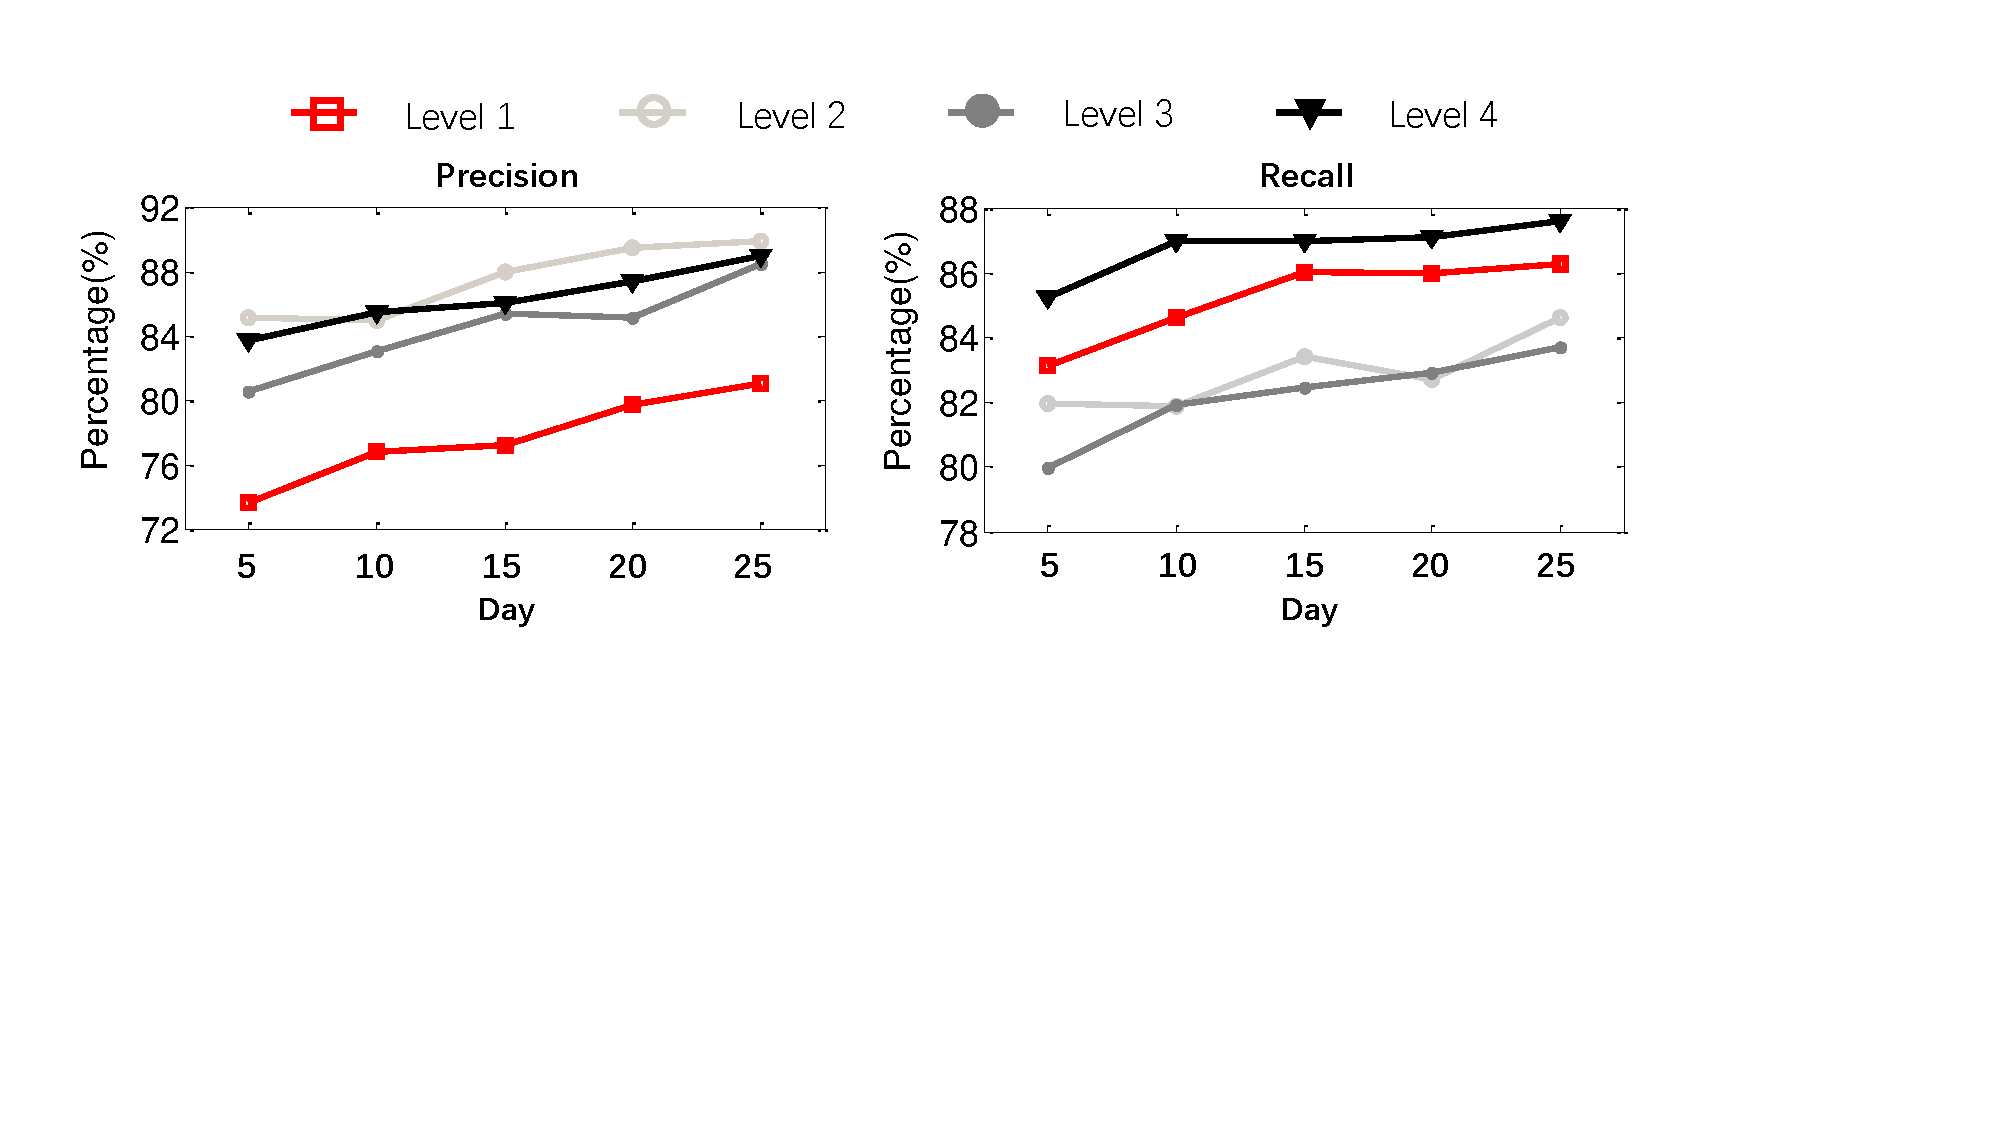
\includegraphics[width=0.9\columnwidth]{./img/performance_under_days1.pdf}
  \caption{Impact of increasing amount of training samples.}
  \label{fig:per_under_train_days}
\end{figure}

\figref{fig:per_under_train_days} illustrates the results for all the 4 blood glucose levels.
The results are averaged over all testing samples as in previous evaluations.
As expected, the precisions and recalls for all the 4 blood glucose levels improve smoothly with the increase of training samples.
The results verify that the challenge (and our motivation to adopt a multi-task learning framework) is the lack of training data.
Note that \sysname is not a replacement of the current CGM devices, but rather, a complement when CGM devices are uncomfortable or inconvenient to wear.
Therefore we envision the training dataset will grow gradually after wearing the CGM device multiple times (at least for diabetes patients), and the overall accuracy will also improve over time as a result.



\subsubsection{Impact of Temporal Gaps}
The blood glucose concentration is correlated with the previous blood glucose levels because of the control loop of the glucose metabolism~\cite{bib:TBE07:Dalla, bib:PE04:Hovorka, bib:IJNMBE16:Oviedo}.
Since \sysname does not rely on the previous blood glucose level as an input, it is natural that the accuracy of \sysname will degrade if there is a long gap between the training and the testing datasets (\ie the training dataset can be outdated).

\begin{figure}[h]
  \centering
  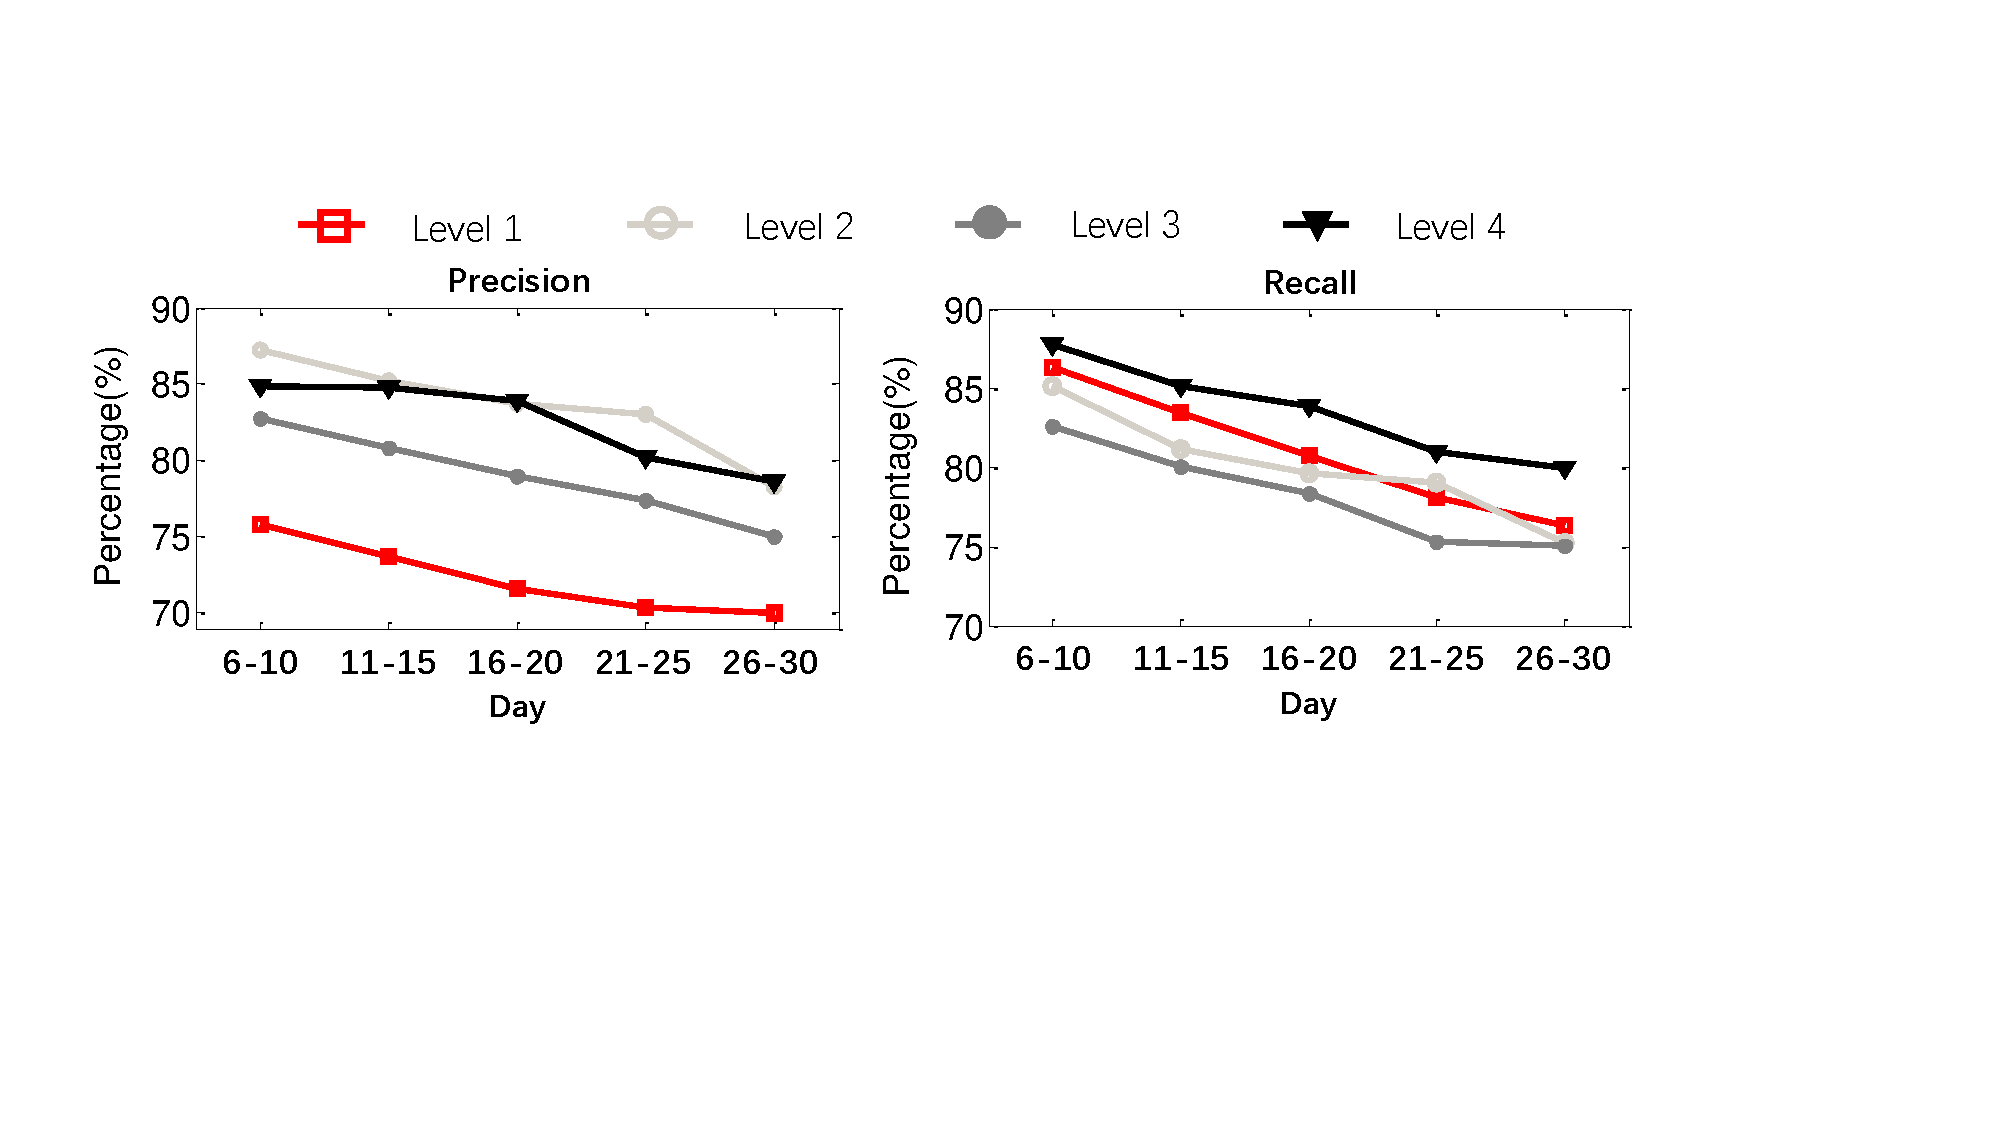
\includegraphics[width=0.9\columnwidth]{./img/Performance_gap1.pdf}
  \caption{Impact of temporal gaps between the training and testing datasets.}
  \label{fig:per_under_various_pred_days}
\end{figure}

\figref{fig:per_under_various_pred_days} plots the overall performance by training using the same 5 days of measurements, and testing on measurements collected on the 6-10th, 11-15th, 16-20th, 21-25th, and 26-30th days, respectively.
As expected, both the precisions and recalls drop moderately with the increase of temporal gaps between the training and the testing datasets, with a maximum decrease of 6.73\% and 7.02\% in average precision and recall after 21-25 days.
Note that \sysname is not designed as a replacement of the commercial CGM devices, but rather a ubiquitous temporary alternative when CGM devices are uncomfortable or inconvenient to wear.
From the results, we recommend \sysname users to put on the CGM device to monitor the blood glucose at least every three weeks.
The data sampled by the CGM will automatically feed into \sysname for a model retraining.




%\subsubsection{Detection Accuracy for Different Groups}
%Fig.~\ref{fig:cmp_groups} illustrates the results of each groups.
%
%\TODO{redraw the figures, no need to include general and personal learning here. show the performance for different health status, gender, age groups, weight groups, \etc, explain why \sysname works better for certain groups, or works well for all groups}.
%
%We also apply general learning approach on the users in same group, and compare the prediction performance of \modelname. Fig.~\ref{fig:cmp_groups}
%shows the results. As is shown, \modelname outperforms the general learning methods in each group, especially the performance of level 1 and level 4. It mainly results by two reasons. On the one hand, the limitation of blood glucose data in each group weakens the capability of temporal dynamic characteristics. On the other hand, the imbalanced distribution of blood glucose data of one group also low the performance down. For example, much more data of level 4 and much less data of level 1 in group 3 (type II diabetes) low down the recall of level 1 and the precision of level 4. It is even hard to be solved by the cost sensitive approach.

